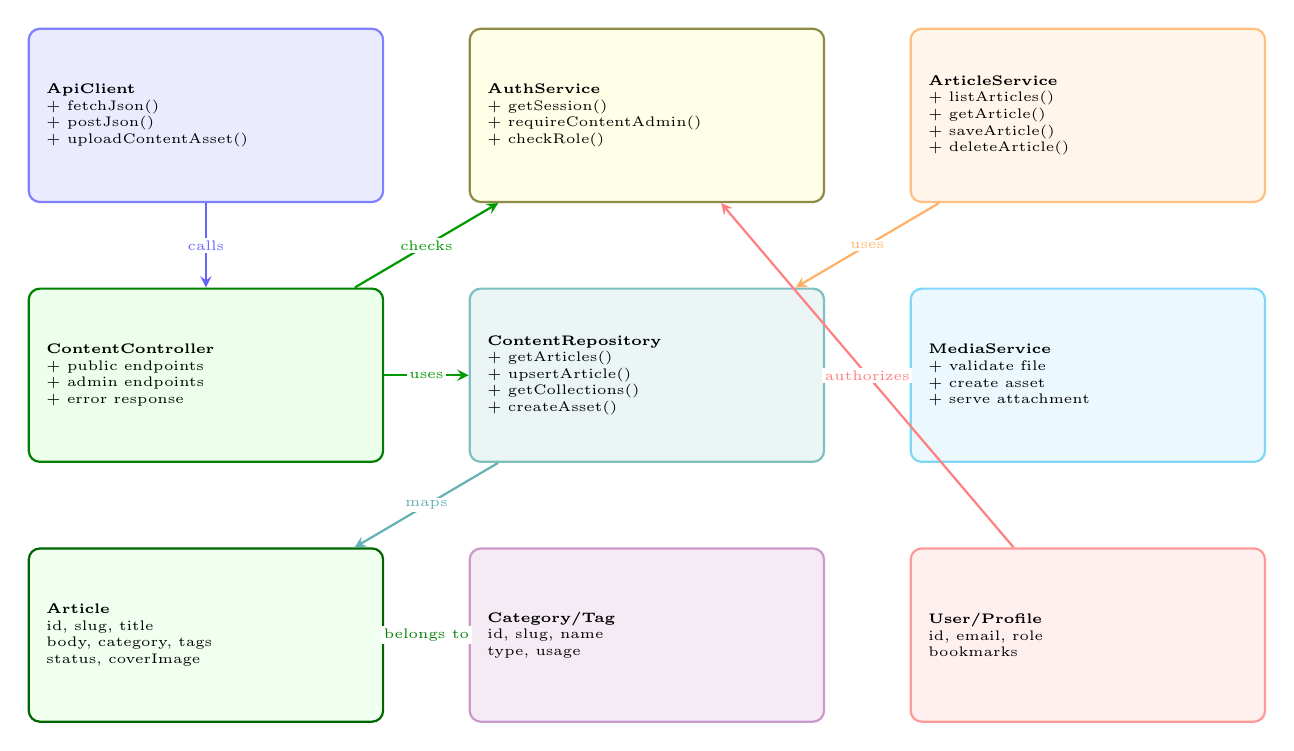
\begin{tikzpicture}[x=1cm,y=1cm,>=stealth,thick]
  \tikzstyle{classbox}=[draw, rounded corners=4pt, minimum width=4.5cm, minimum height=2.2cm,
    text width=4.05cm, align=left, font=\tiny]
  \tikzstyle{rel}=[font=\tiny, fill=white, inner sep=1pt]

  % Frontend / Client layer
  \node[classbox, fill=blue!8, draw=blue!50] (api) at (0,5.6) {\textbf{ApiClient}\\+ fetchJson()\\+ postJson()\\+ uploadContentAsset()};
  \node[classbox, fill=yellow!10, draw=yellow!50!black] (auth) at (5.6,5.6) {\textbf{AuthService}\\+ getSession()\\+ requireContentAdmin()\\+ checkRole()};
  \node[classbox, fill=orange!8, draw=orange!50] (articleService) at (11.2,5.6) {\textbf{ArticleService}\\+ listArticles()\\+ getArticle()\\+ saveArticle()\\+ deleteArticle()};

  % Controller / Repository layer
  \node[classbox, fill=green!8, draw=green!50!black] (controller) at (0,2.3) {\textbf{ContentController}\\+ public endpoints\\+ admin endpoints\\+ error response};
  \node[classbox, fill=teal!8, draw=teal!50] (repo) at (5.6,2.3) {\textbf{ContentRepository}\\+ getArticles()\\+ upsertArticle()\\+ getCollections()\\+ createAsset()};
  \node[classbox, fill=cyan!8, draw=cyan!50] (media) at (11.2,2.3) {\textbf{MediaService}\\+ validate file\\+ create asset\\+ serve attachment};

  % Domain entity layer
  \node[classbox, fill=green!6, draw=green!40!black] (article) at (0,-1.0) {\textbf{Article}\\id, slug, title\\body, category, tags\\status, coverImage};
  \node[classbox, fill=violet!8, draw=violet!40] (category) at (5.6,-1.0) {\textbf{Category/Tag}\\id, slug, name\\type, usage};
  \node[classbox, fill=red!6, draw=red!40] (user) at (11.2,-1.0) {\textbf{User/Profile}\\id, email, role\\bookmarks};

  % Relationships
  \draw[->, blue!60] (api) -- node[rel] {calls} (controller);
  \draw[->, green!60!black] (controller) -- node[rel] {checks} (auth);
  \draw[->, green!60!black] (controller) -- node[rel] {uses} (repo);
  \draw[->, orange!60] (articleService) -- node[rel] {uses} (repo);
  \draw[->, cyan!60] (media) -- node[rel] {stores} (repo);
  \draw[->, teal!60] (repo) -- node[rel] {maps} (article);
  \draw[->, green!50!black] (article) -- node[rel] {belongs to} (category);
  \draw[->, red!50] (user) -- node[rel] {authorizes} (auth);
\end{tikzpicture}
